\documentclass[a5paper,12pt,draft,titlepage]{scrartcl}

\usepackage[ngerman]{babel}
\usepackage[T1]{fontenc}
\usepackage[ansinew]{inputenc}
\usepackage{lmodern}
\usepackage{graphicx}

\begin{document}

\pagestyle{empty}
\title{Kurzanleitung \textsc{Detroit Electric Car}}
\author{Yanick Frei}

\maketitle
\begin{figure}[h]
	\centering
		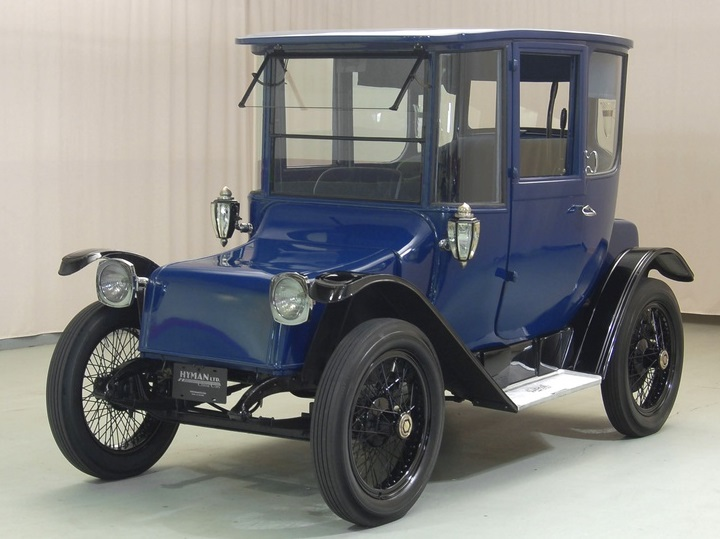
\includegraphics[width=0.60\textwidth]{Bilder/Titelbild.jpg}
\end{figure}

In diesem Dokument soll kurz auf den \textsc{Detroit} eingegangen werden, insbesondere auf dessen Bedienung. F�r weitere Informationen, insbesondere fachliche Fragen, sei auf den Fachbericht zum Umbau des Fahrzeuges verwiesen. Wir w�nschen nun viel Spass beim Lesen und vor allem beim Fahren!

\tableofcontents \newpage

\section{Informationen zum Fahrzeug}

\section{Aufladen den Batterie}
Das Aufladen der Batterie geschieht in mehreren Schritten (\textit{kursive} Vorg�nge werden dabei automatisch von der Batteriesteuerung �bernommen):

\begin{enumerate}
\setlength{\itemsep}{10pt}
	\item Das Fahrzeug wird abgestellt und im Idealfall mit der Handbremse gesichert.
	\item Das 230V-Ladekabel wird eingesteckt und an der Steuerbox der Schalter auf \textsc{Ein} geschaltet.
	\item \textit{Das 12V-Netz des Fahrzeuges wird automatisch unterbrochen, womit der Hauptschalter nicht mehr eingeschaltet und losgefahren werden kann. Das soll ein versehentliches Losfahren w�hrend dem Laden verhindern.}
	\item \textit{Sind die Batterien nicht voll, wird automatisch der Ladephase gestartet. Bei komplett entleerter Batterie kann diese Phase bis zu 10 Stunden dauern.}
	\item \textit{Bereits w�hrend der Ladephase beginnt die Balancingphase, welche eine gleichm�ssige Ladung der Zellen sicher stellt. Diese Phase sollte im Normalfall nicht viel l�nger dauern als die Ladephase (das finale Balancing kann erst nach dem Vollladen der Zellen durchgef�hrt werden)}
	\item Nach dem Entfernen des Netzkabels wird das 12V-Netz wieder freigegeben, was ein Einschalten des Fahrzeugs erm�glicht.
\end{enumerate}

Der gesamte Ladevorgang inklusive Balancing sollte im Normalfall h�chstens 12 Stunden dauern (bei komplett leerer Batterie). Das Ende der Ladephase kann einfach dadurch erkennt werden, dass beide Ladeger�te in der Front des Fahrzeugs ihre L�fter abgestellt haben. Wenn m�glich sollte ab dann der Balancingphase noch zwei Stunden Zeit gegeben werden. Falls dies nicht m�glich ist, kann dies jedoch auch durch eine l�ngere Balancingphase beim n�chsten Ladevorgang kompensiert werden.

\section{Bewegen des Fahrzeuges}

\section{Bekannte Schwachstellen}


\end{document}
